\chapter{Mathematical foundations}\label{chap:math}

Before I delve into the details of the visual-inertial relative navigation algorithm, it is important to establish theoretical foundations. This chapter summarizes the mathematical preliminaries that are essential for understanding how the algorithm works. It covers key concepts about coordinate systems and camera projection and introduces an alternative method of rotation representation. 

In this paper, filter-related mathematics uses 3+1 frames: Earth (E), node (N)-, body (B), and camera (C) frame. The purpose of the node frame is mentioned later which is connected to relative navigation applications, but currently, there is not applied such a frame in my approach. The Earth alias localization, body, and camera frames are utilized in the calculations of the algorithm. The frames are shown in Figure~\ref{fig:coord-sys}. 
\begin{figure}[!ht]
    \centering
    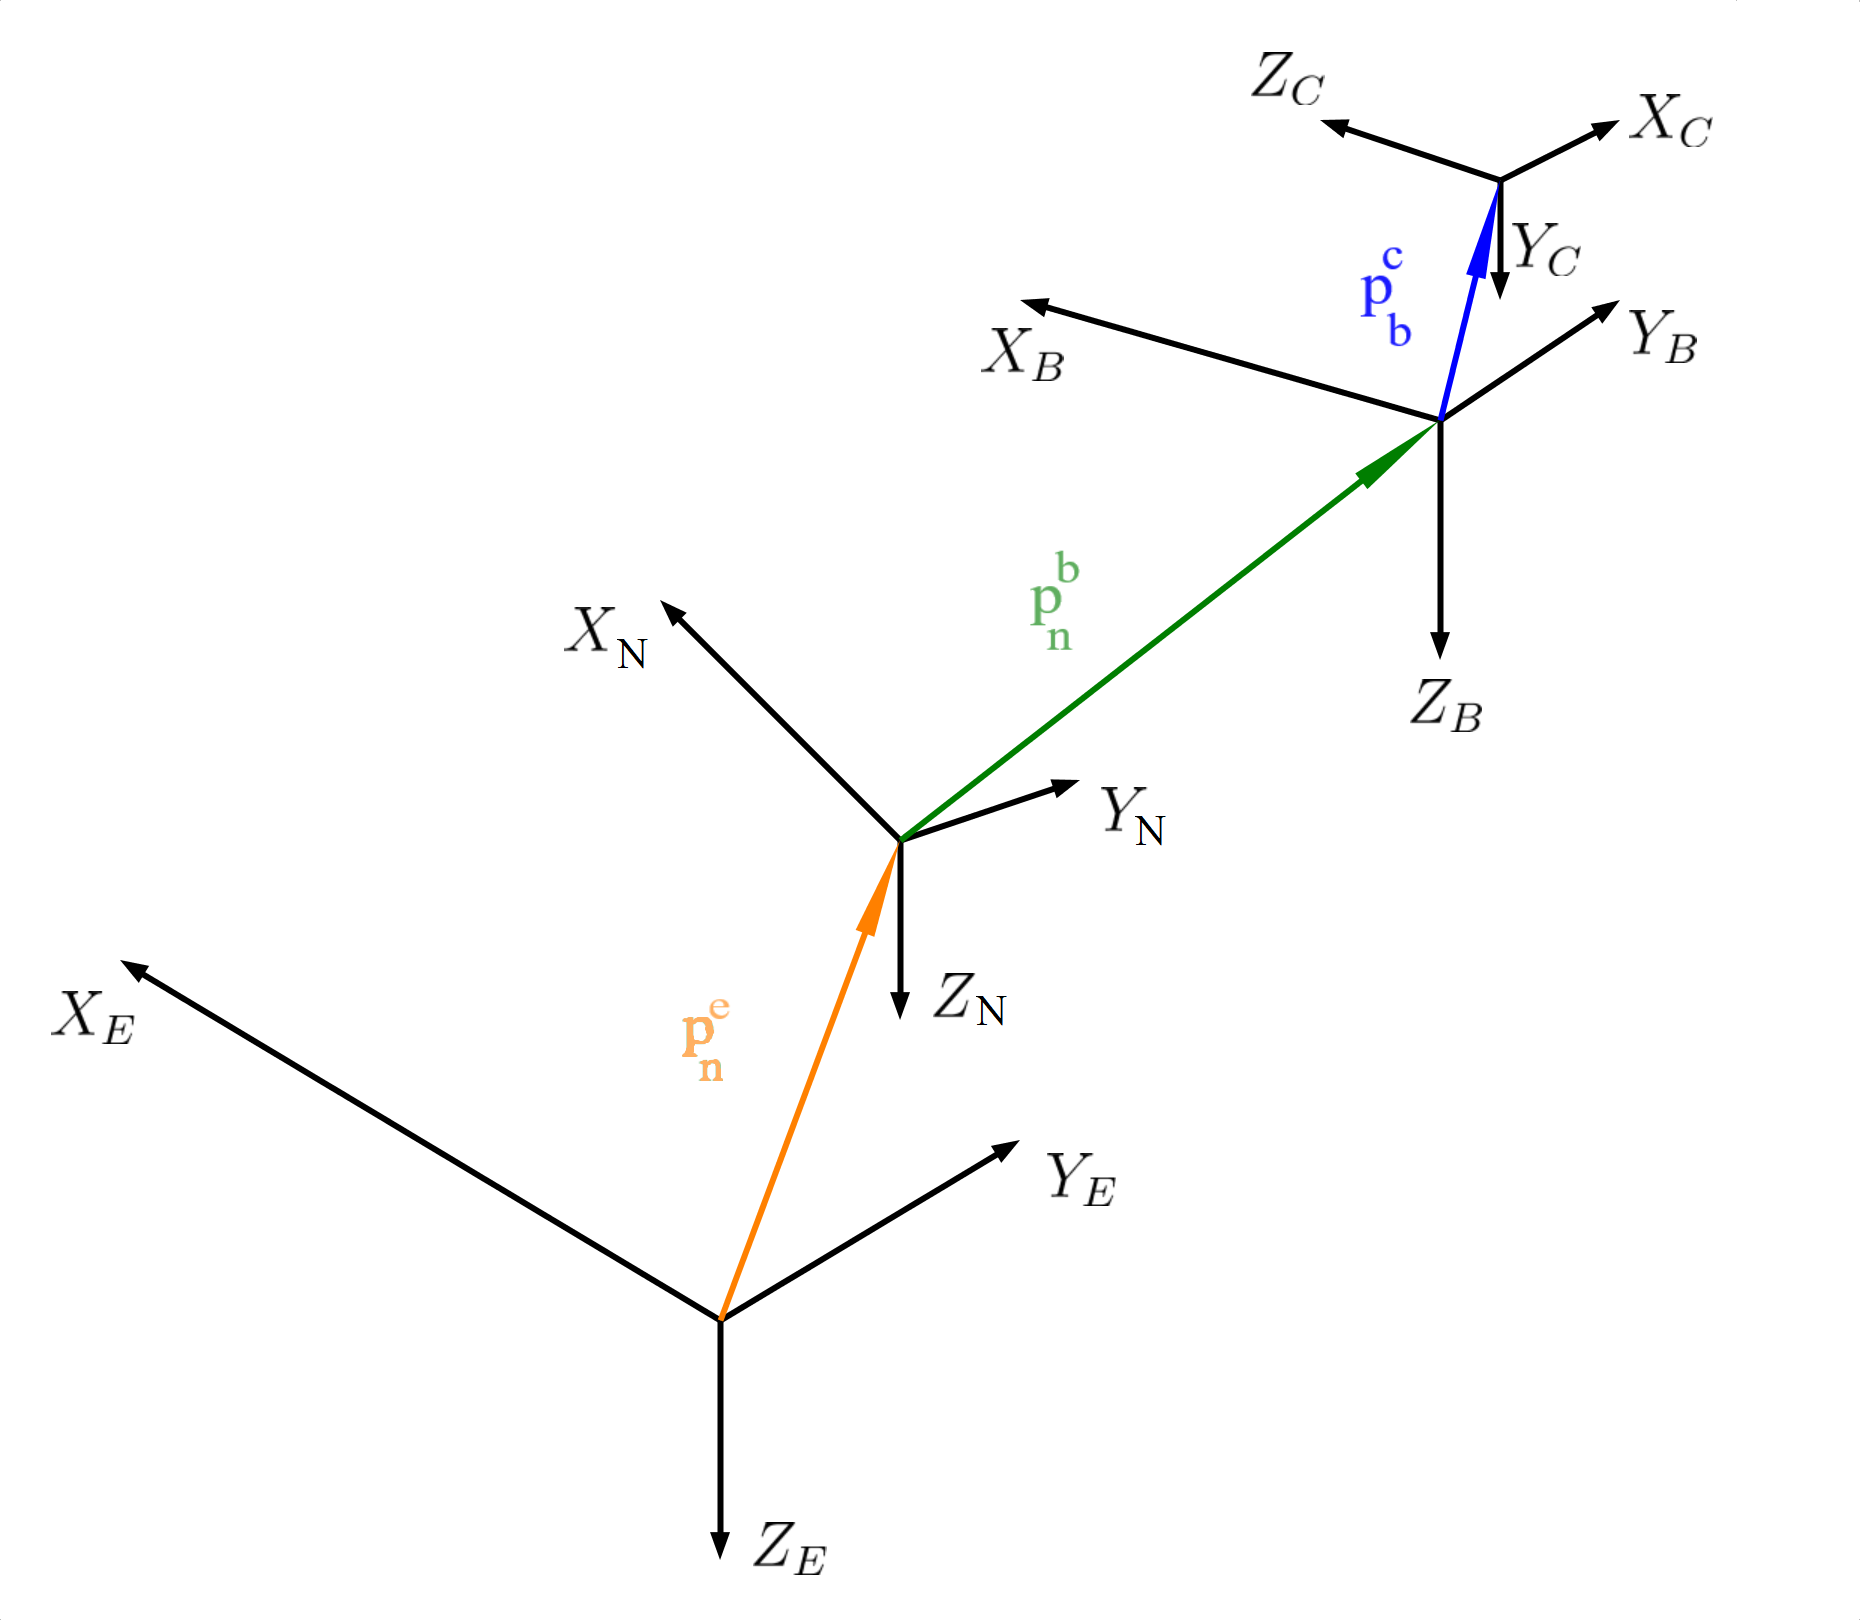
\includegraphics[width=0.8\textwidth]{figures/Coord_sys.png}
    \caption{Applied coordinate systems}\label{fig:coord-sys}
\end{figure}

The Earth frame is an Earth fixed frame and in this application, the North-East-Down (NED) coordinate system was chosen for this purpose because it can be used as an inertial frame in such UAV applications where the vehicle covers only a few \si{\kilo\meter}s\footnote{If flight trajectories remain short the curvature of the Earth can be neglected.}. In the following, the filter-related mathematical notation uses n, b, and c for inertial, body, and camera frames.

\section{Navigation frames}

 The purpose of using different kinds of frames is to facilitate the kinematic modeling of UAVs. To effectively study UASs, it is crucial to comprehend the relative orientation and translation of different coordinate systems. Multiple frames are required for several reasons:
\begin{itemize}
    \item 
    The motion of the aircraft is most easily described in a body-fixed frame, however, Newton's equations of motion are derived relative to an inertial reference frame.
    \item 
    The body-fixed frame is also used to express the aerodynamic forces and moments that affect the aircraft.
    \item
    On-board sensors such as accelerometers and gyroscopes provide measurements concerning the body frame in the case of strap-down IMUs.
    \item 
    Finally, the mission requirements of the aircraft, \eg{} flight path require a global (absolute) frame.
\end{itemize}

\subsection{North-East-Down reference frame}

The NED coordinate system has emerged as a standard in UAV applications over limited distances, typically spanning a few kilometers. Notably, this reference frame is conventionally anchored to a stationary point on Earth, affording its use as an inertial reference frame in analytical computations. It can be seen in Figure~\ref{fig:NED} compared to the globe and Earth-centered Earth-fixed (ECEF) coordinate system. Consistent with its name, the NED system aligns its X-axis with the geographic north, its Y-axis with the east, and its Z-axis points inwards to the Earth. Its X-Y plane is the local tangent plane of the Earth's ellipsoid.

\begin{figure}[!ht]
    \centering
    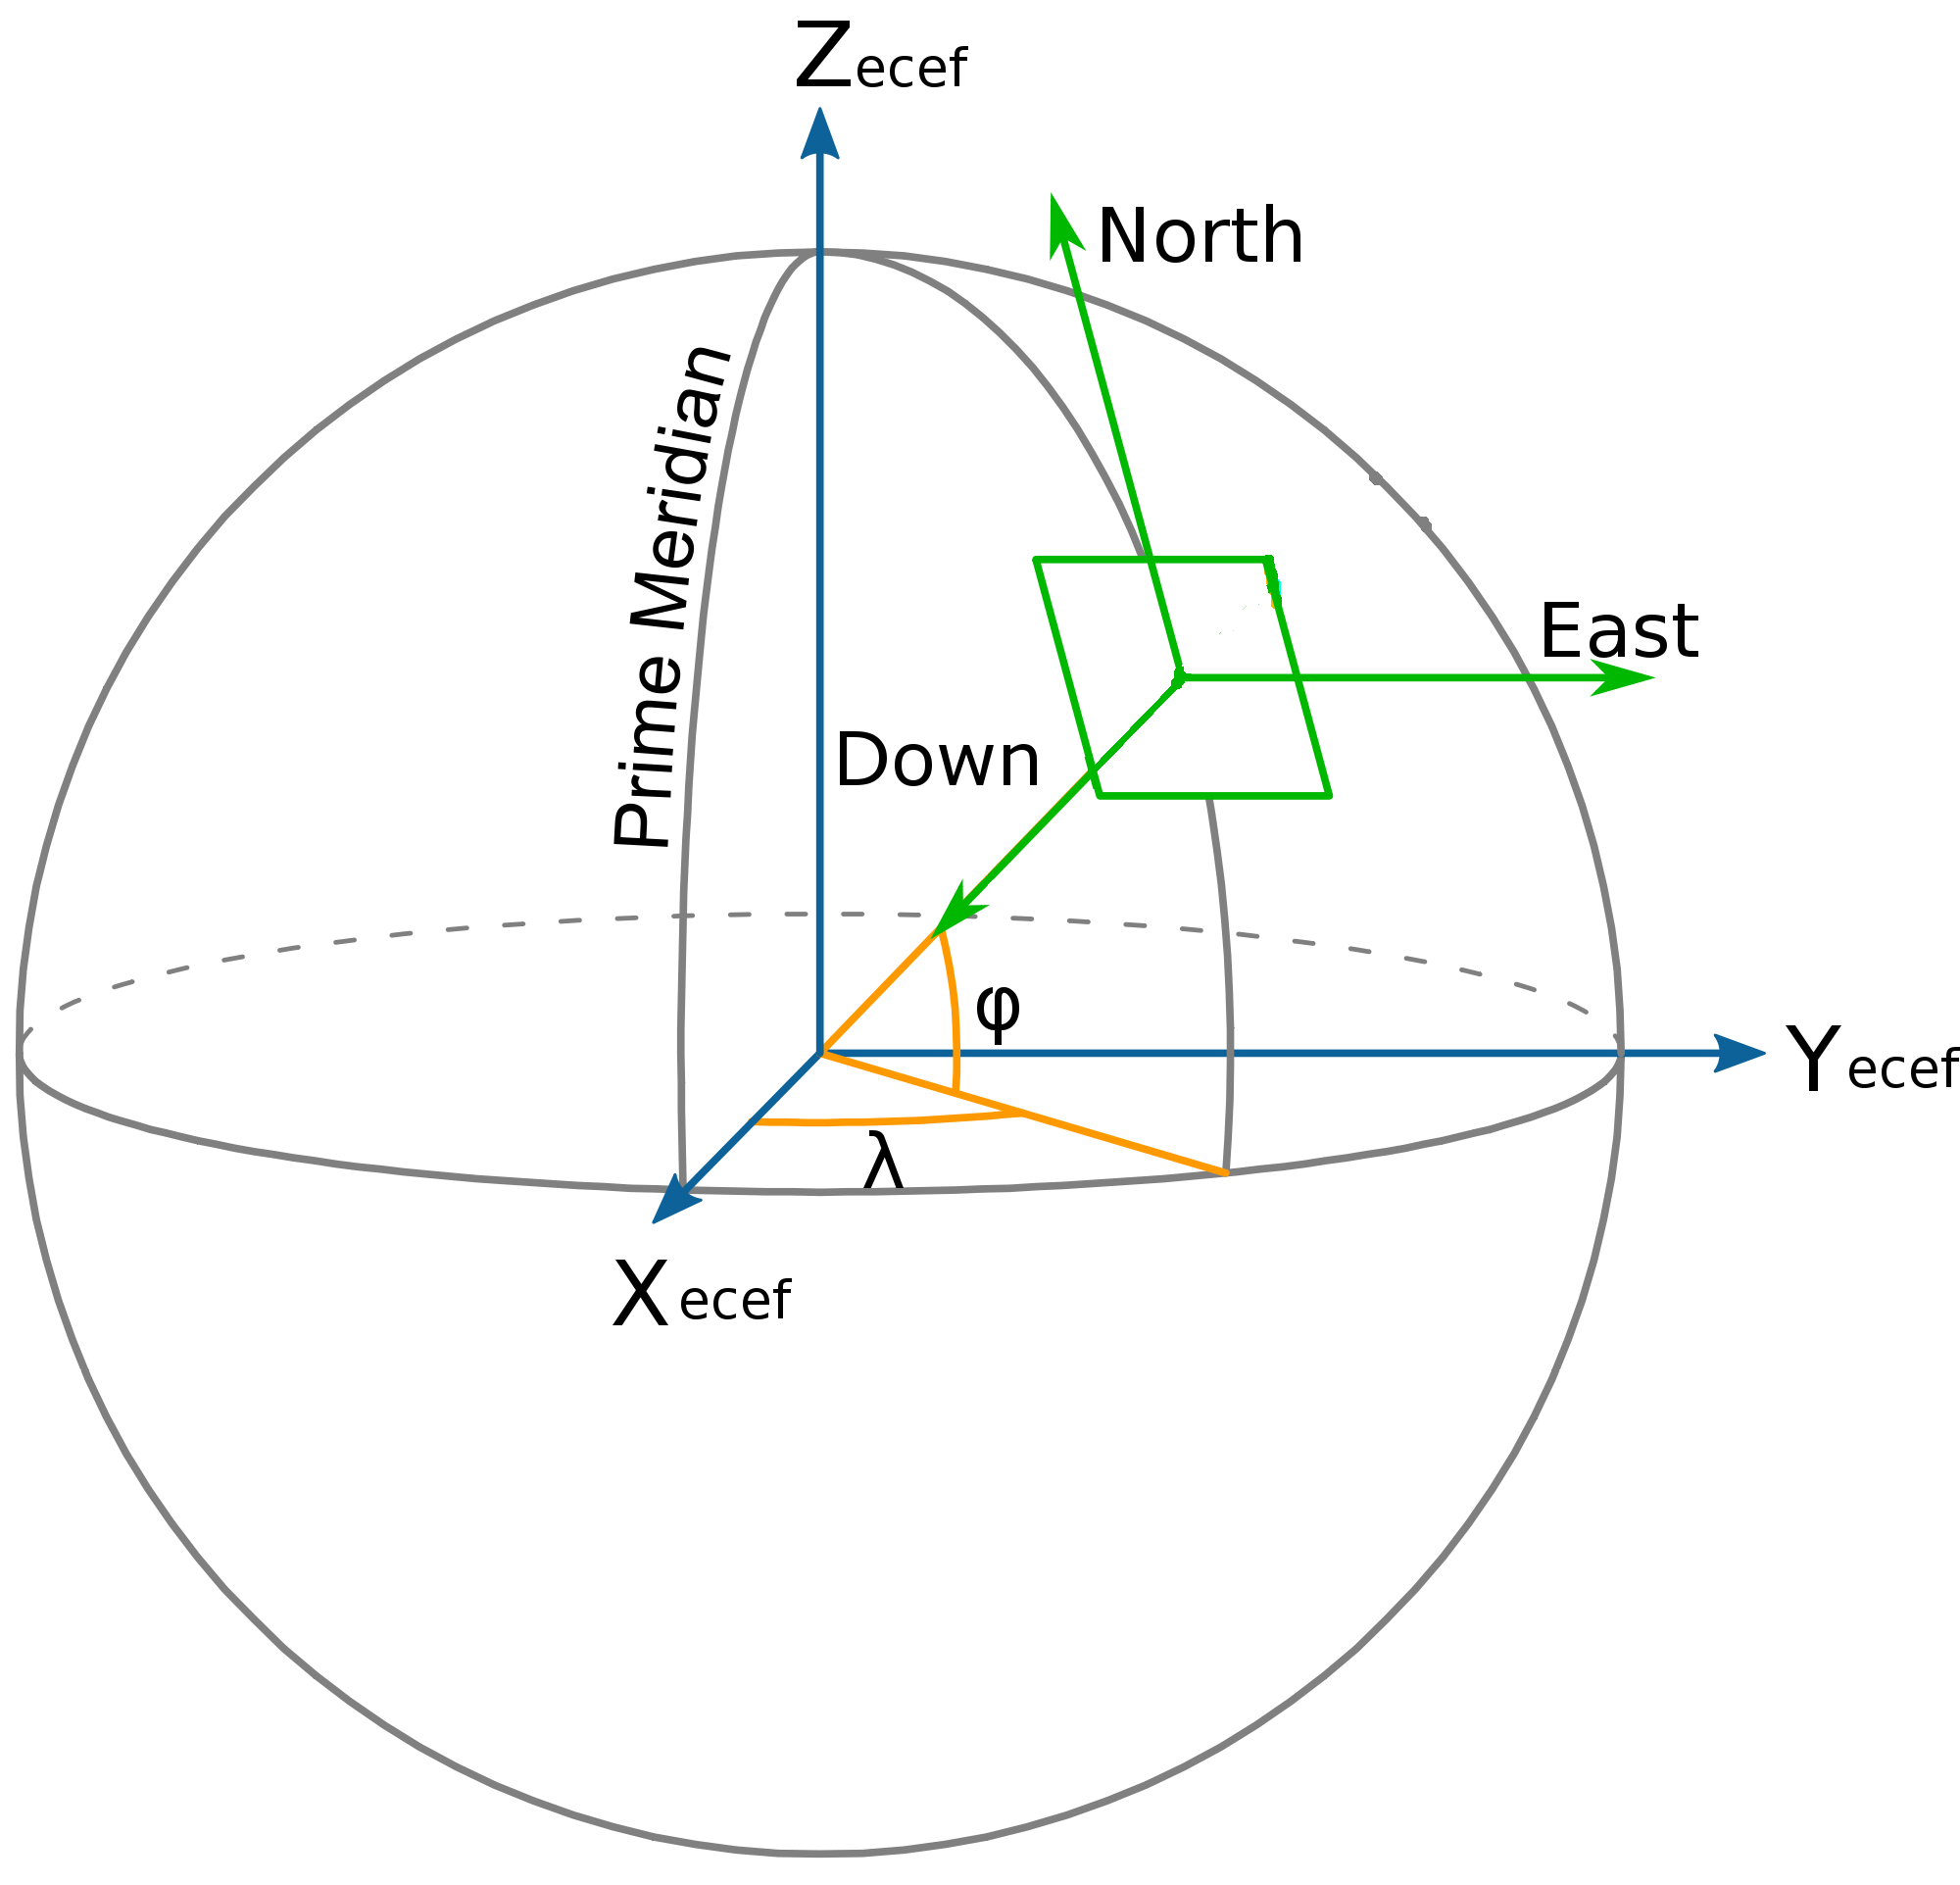
\includegraphics[width=0.8\textwidth]{figures/NED.png}
    \caption{NED coordinate system~\cite{gps_navigation_slide}}\label{fig:NED}
\end{figure}

The front end of relative navigation methods adopts the node coordinate system as an inertial frame, a crucial precondition for the functioning of the filter. For example in~\cite{rel-nav} the node frame remains locally fixed and undergoes redeclaration whenever they perform a measurement update. The back end is responsible for producing global estimates, such as NED coordinates, utilizing the outcomes yielded by the filter.

\subsection{Body frame}

In the kinematic equations, quantities are usually described in inertial or body frame, therefore it is crucial to understand properly how the body frame is defined and how can the relation can be accounted to the inertial frame. The origin is aligned with the center of the aircraft's mass, and worth mentioning the fact in realizations the IMU is placed here. The axes of the body frame are defined as follows: the X-axis points out the nose of the aircraft, the Y-axis points out the right wing and the Z-axis points downwards.

Once the coordinate system has been defined, it is necessary to mention the relation to the inertial frame. The most commonly applied approach to obtain the orientation of the aircraft in the NED system is to express it with Euler angles which means three rotations one after another. Defining the Euler angles I use the same terminology as in~\cite{EKF-UAS-2}, their approach is to introduce three additional coordinate systems: vehicle, vehicle-1, and vehicle-2. They are shown in Figure~\ref{fig:vehicle}-\ref{fig:body}.

\begin{figure}[!ht]
    \centering
    \begin{subfigure}{0.38\textwidth}
        \centering
         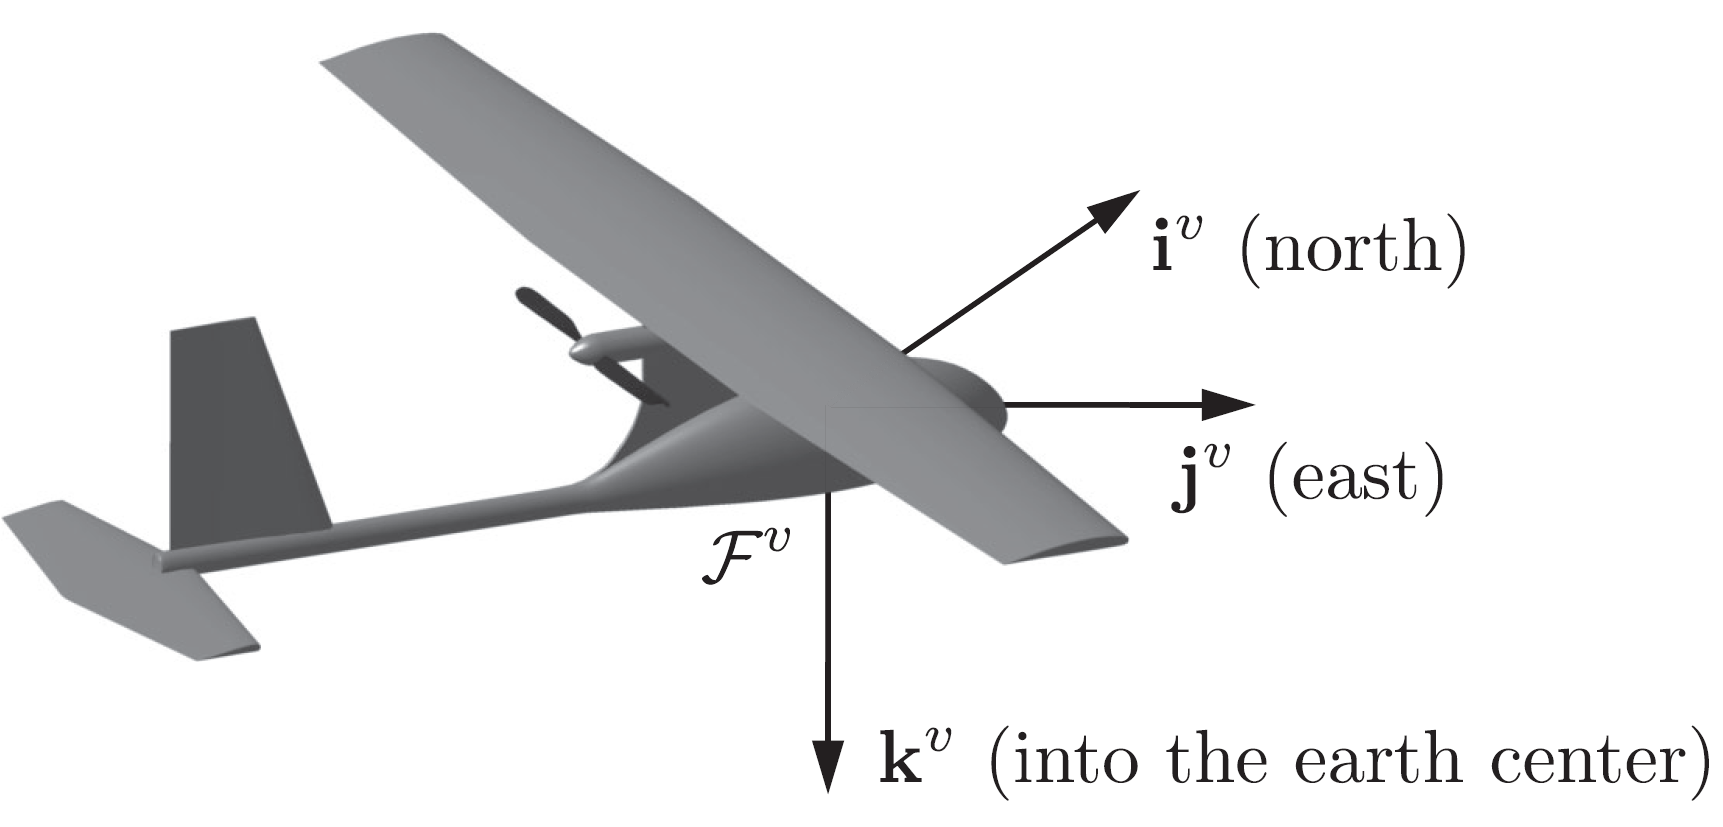
\includegraphics[width=\textwidth]{figures/vehicle.png}
         \caption{Vehicle}\label{fig:vehicle}
    \end{subfigure}
    \begin{subfigure}{0.38\textwidth}
        \centering
         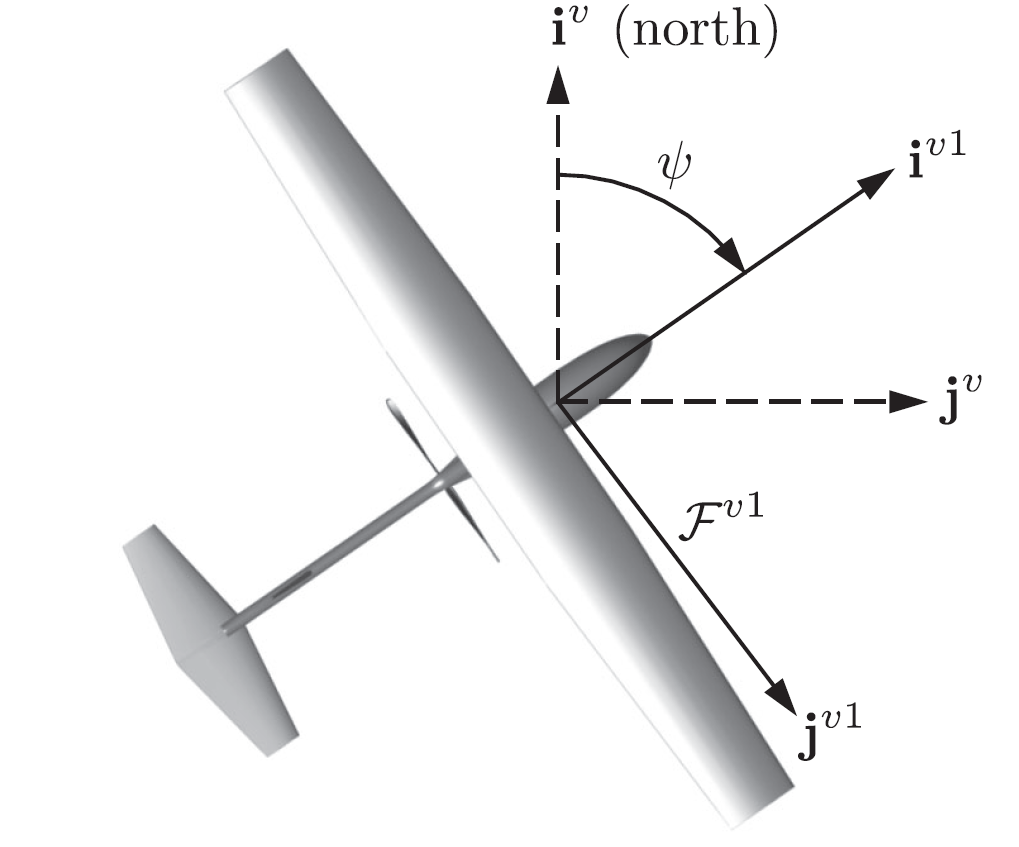
\includegraphics[width=\textwidth]{figures/vehicle-1.png}
         \caption{Vehicle-1}\label{fig:vehicle-1}
    \end{subfigure}
    \begin{subfigure}{0.38\textwidth}
        \centering
         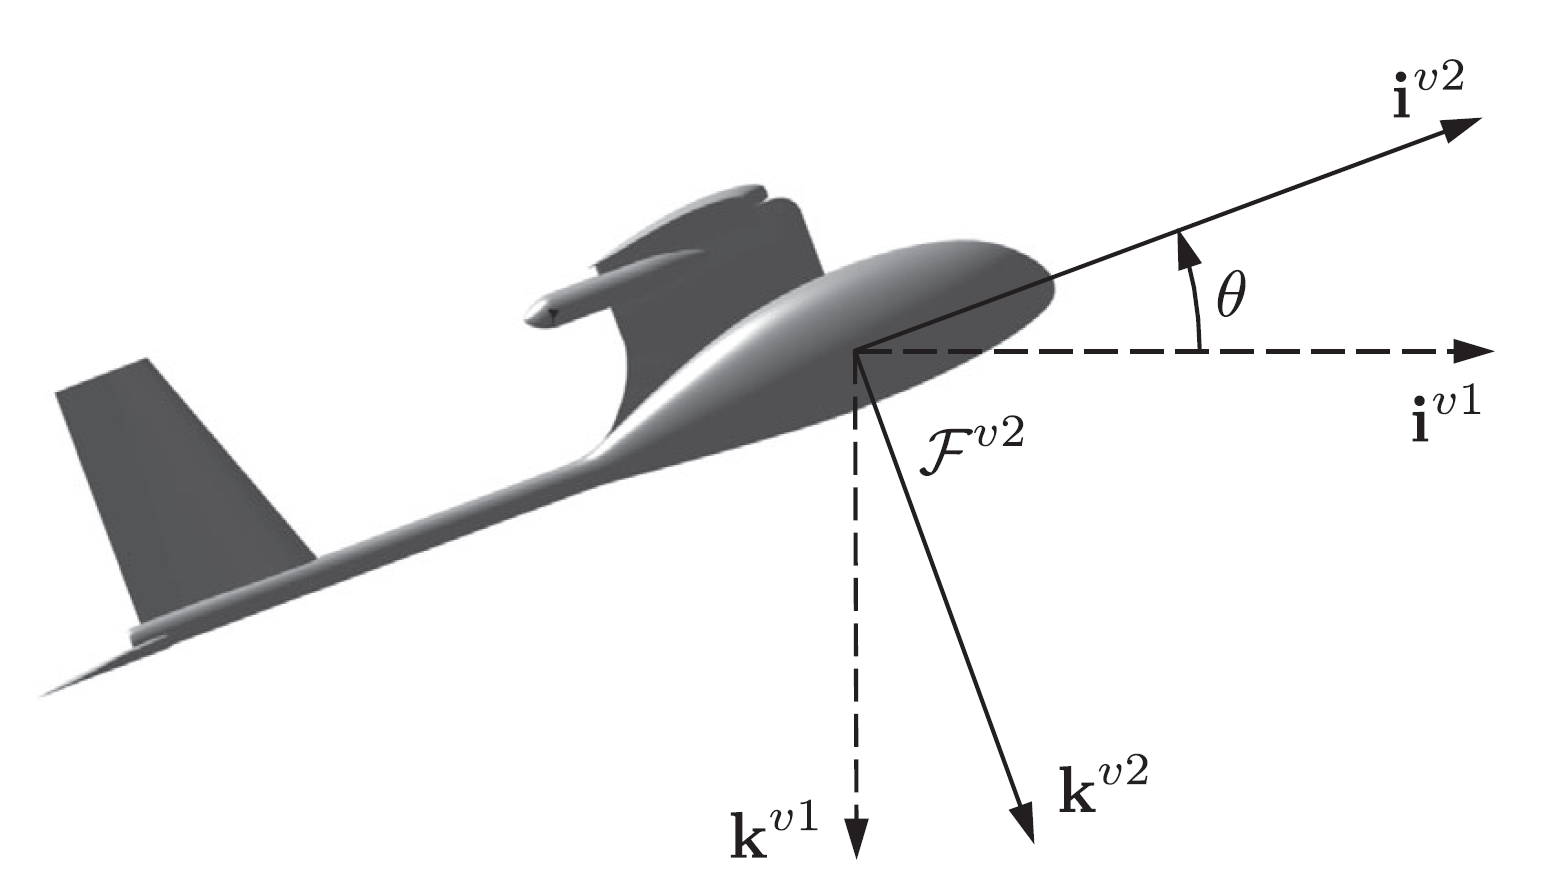
\includegraphics[width=\textwidth]{figures/vehicle-2.png}
         \caption{Vehicle-2}\label{fig:vehicle-2}
    \end{subfigure}
    \begin{subfigure}{0.38\textwidth}
        \centering
         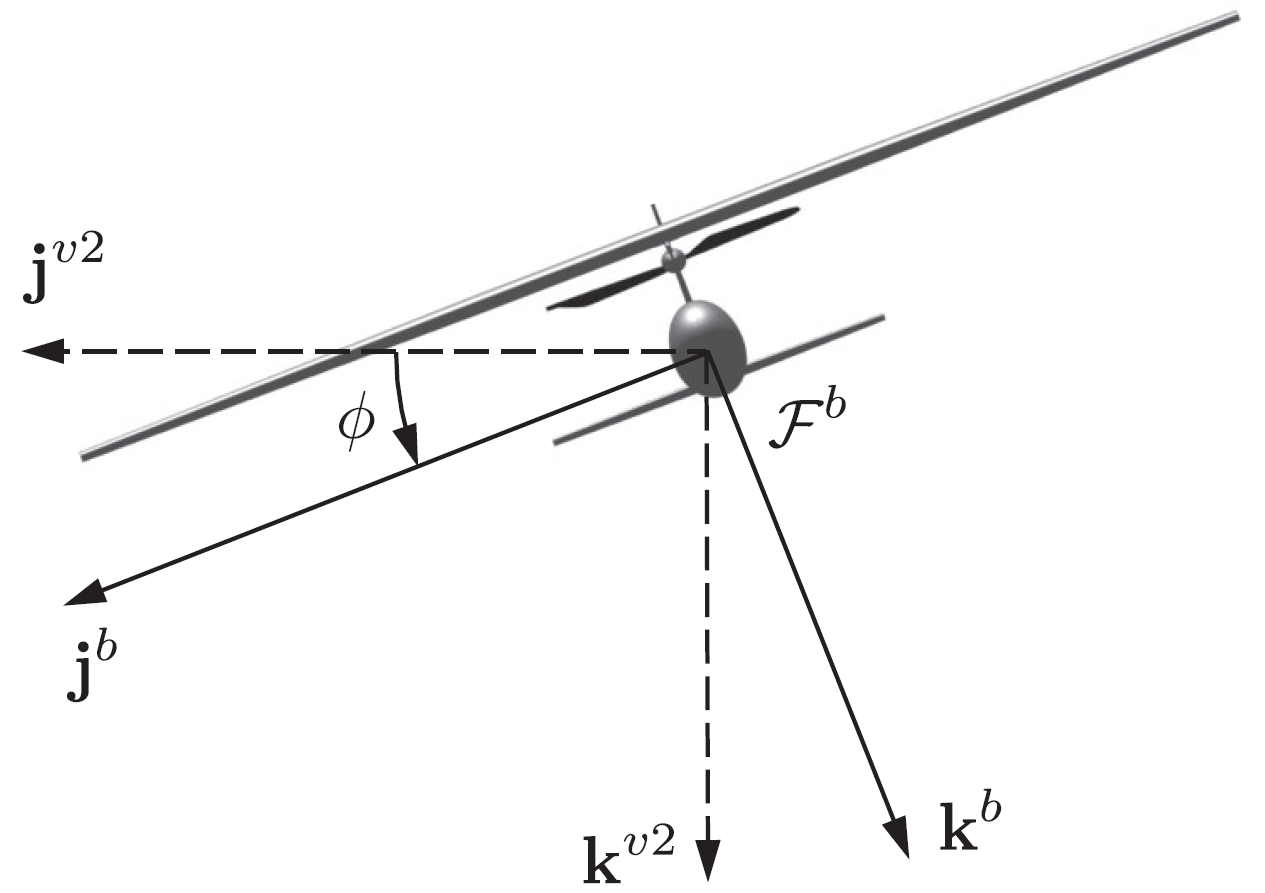
\includegraphics[width=\textwidth]{figures/body.png}
         \caption{Body frame}\label{fig:body}
    \end{subfigure}\label{fig:frames}
    \caption{Frames to define Euler angles (\cite{EKF-UAS-2}: pages 13--15, Figures 2.4--2.7)}
\end{figure}

The vehicle frame is the NED coordinate system with shifted origin into the center of mass, vehicle-1 frame is rotated with the yaw angle ($\psi$)  around the Z-axis of the vehicle frame, vehicle-2 frame is rotated with pitch angle ($\theta$) around the Y-axis of vehicle-1 frame, and body frame is rotated with roll angle ($\phi$) around the X-axis of vehicle-2 frame. To summarize, the resulting rotation can be defined as:

\begin{equation}
\begin{aligned}
    \mathbf{R}_{BV}(\phi,\theta,\psi)&=\mathbf{R}_{BV_2}(x,\phi)\mathbf{R}_{V_2V_1}(y,\theta)\mathbf{R}_{V_1V}(z,\psi) \\
    &=
    \begin{bmatrix}
        C_\theta C_\psi & C_\theta S_\psi & -S_\theta \\
        S_\phi S_\theta C_\psi - C_\phi S_\psi & S_\phi S_\theta S_\psi + C_\phi C_\psi & S_\phi C_\theta \\
        C_\phi S_\theta C_\psi + S_\phi S_\psi & C_\phi S_\theta S_\psi - S_\phi C_\psi & C_\phi C_\theta
    \end{bmatrix}, 
\end{aligned}
\label{eq:euler-angles}
\end{equation}

where $C_\alpha$ is shorthand for $\cos(\alpha)$ and $S_\alpha$ for $\sin(\alpha)$.

Finally, I want to mention the usage of homogeneous transformation which is widespread regarding vision-based applications, thanks to the fact it allows the calculation of three-dimensional (3-D) coordinates from one frame to another with a single matrix multiplication. The homogeneous transformation between two frames requires the usage of both orientation and position relative to each other. For example, considering body-to-earth transformation $\mathbf{R}_{NB}\equiv\mathbf{R}_{VB}$ accounts for rotation, and $\mathbf{p}_n^b$ is the translational vector describing the position of the body frame's origin in NED coordinates. Then the homogeneous transformation can be expressed as:
\begin{equation}
    \mathbf{H}_{NB}=\begin{bmatrix}
        \mathbf{R}_{NB} & \mathbf{p}_n^b \\
        \mathbf{0}^T & 1
    \end{bmatrix}
    \label{eq:hom-e2b}
\end{equation}

The transformation can be applied as:
\begin{equation}
    \mathbf{H}_{NB}\begin{bmatrix}
        \mathbf{v}_b \\ 1
    \end{bmatrix}=\begin{bmatrix}
        \mathbf{R}_{NB} & \mathbf{p}_n^b\\
        \mathbf{0}^T & 1
    \end{bmatrix}\begin{bmatrix}
        \mathbf{v}_b \\ 1
    \end{bmatrix}=\begin{bmatrix}
    \mathbf{R}_{NB}\mathbf{v}_b+\mathbf{p}_n^b \\ 1
    \end{bmatrix} = \begin{bmatrix}
        \mathbf{v}_n \\ 1
    \end{bmatrix}
\end{equation}

\section{Camera frames}

It is important to say a few words about camera-related frames and transformation since camera pictures are used to improve the navigation algorithm. A camera- and an image coordinate system are distinguished, the first one is interpreted in 3-D, and its origin is aligned with the camera center. The image coordinate system spans two dimensions and it is usually one of the XY-planes of the camera frame. 

To mathematically model the projection, the camera's intrinsic and extrinsic parameters have to be used. For the pinhole model, the intrinsic parameters of the camera are focal length ($f$), principal point ($p_x$, $p_y$), and a constraint for the visible points is the field of view (FOV) or image size. Extrinsic parameters describe the position and orientation of the camera in the inertial frame.

\subsection{Camera system}

It is very important to determine the transformation from body-to-camera system with sufficient accuracy. Generally, the camera can not be placed in the body center, therefore the transformation requires a position that is described compared to the body frame and detonated as $\mathbf{p}_{b}^c$. As regards the orientation, since navigation happens concerning the surroundings an at least partially downward-facing camera is mandatory, thus introducing a rotation around the Y-axis of the body frame. Furthermore, the axes of the camera system are defined differently, than the axes of the body frame, therefore an additional operation is essential to change the axes. Figure~\ref{fig:camera-system} shows the camera frame and the image plane. 

\begin{figure}[!ht]
    \centering
    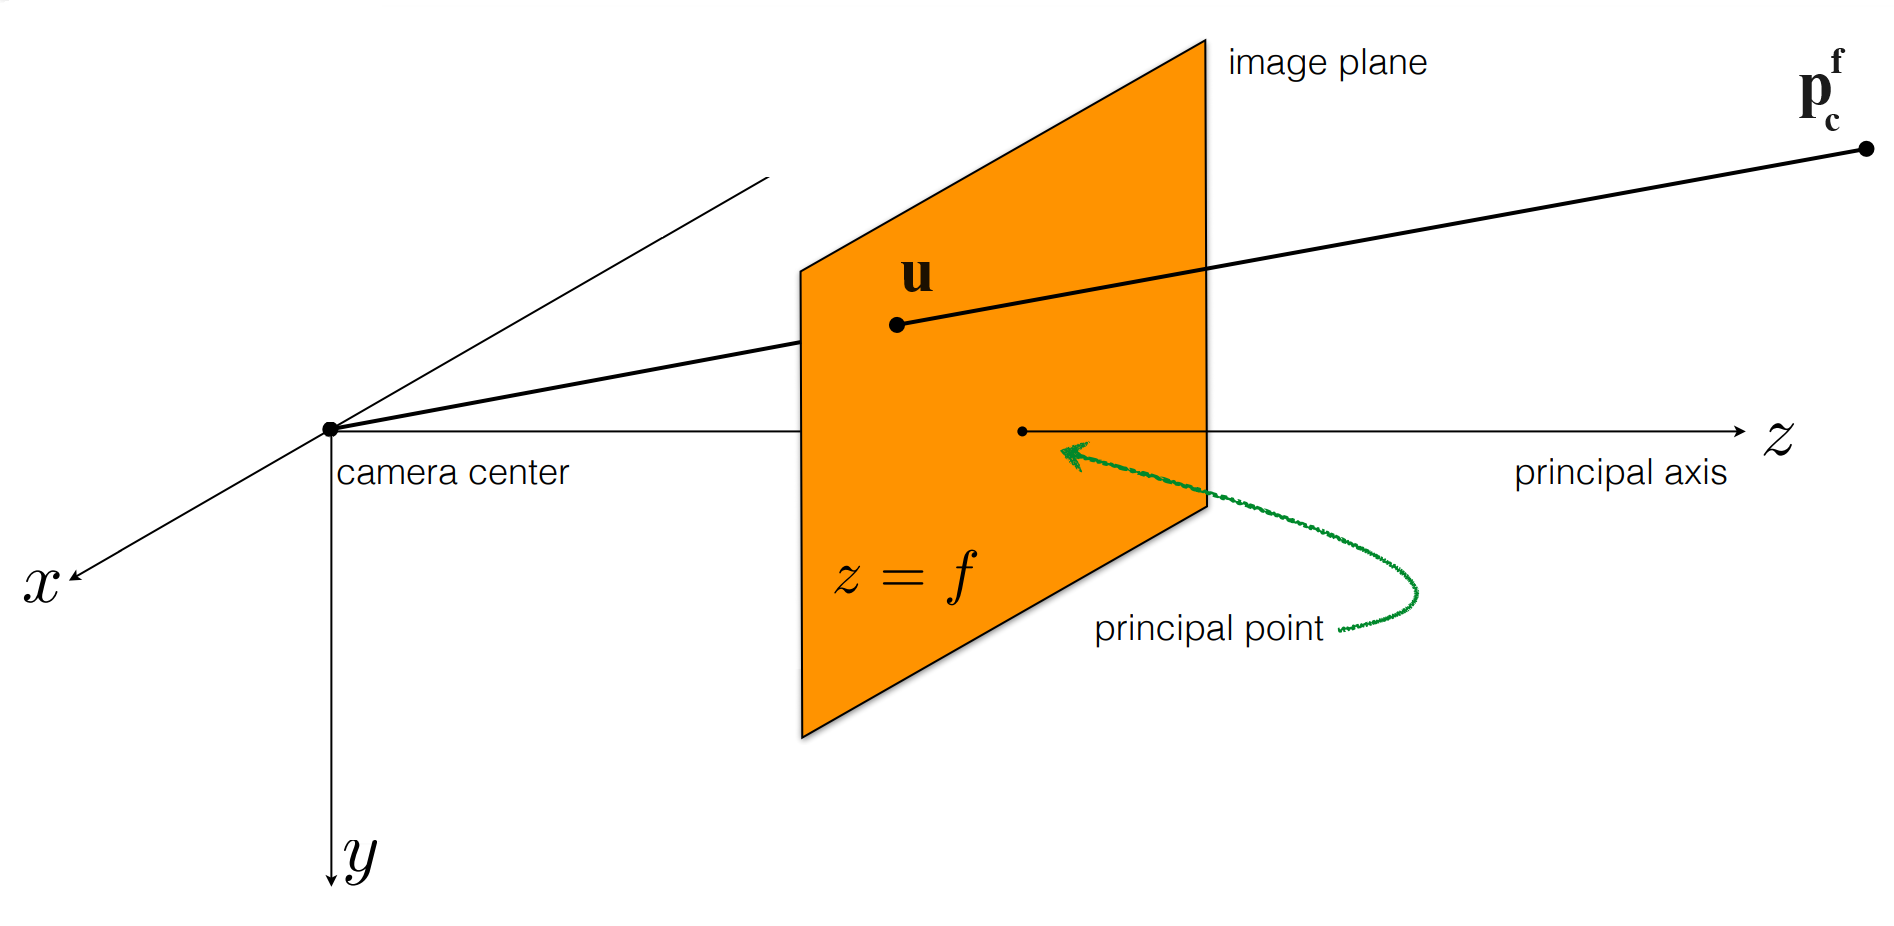
\includegraphics[width=\textwidth]{figures/camera.png}
    \caption{Camera and image system (\cite{camera-matrix-slide}: page 7)}\label{fig:camera-system}
\end{figure}

The axes of the image system are aligned with the camera system's X and Y axes but shifted with the principal point. The principal point is usually near to the center of the image and shifting with it results in a top left corner origin of the pixel coordinate system.

The axes swap operation of the rotated body frame should be transformed as outlined below: $\mathbf{i}_b'=\mathbf{k}_c$, $\mathbf{j}_b'=\mathbf{i}_c$ and $\mathbf{k}_b'=\mathbf{j}_c$, where $\mathbf{i}$, $\mathbf{j}$ and $\mathbf{k}$ are unit vectors along X-, Y- and Z-axis respectively. Utilizing the linear transformations the whole transformation from body-to-camera frame:
\begin{equation}
\begin{aligned}
    \mathbf{T}_{CB}=\mathbf{S}\mathbf{R}_{CB}(y,-\beta) &= \begin{bmatrix}
            0 & 1 & 0 \\
            0 & 0 & 1 \\
            1 & 0 & 0 \\
        \end{bmatrix}
        \begin{bmatrix}
            \cos(\beta) & 0 & -\sin(\beta) \\
            0 & 1 & 0 \\
            \sin(\beta) & 0 & \cos(\beta) \\
        \end{bmatrix} \\ &= \begin{bmatrix}
            0 & 1 & 0 \\
            \sin(\beta) & 0 & \cos(\beta) \\
            \cos(\beta) & 0 & -\sin(\beta) \\
        \end{bmatrix},
\end{aligned}
\end{equation}

where $\mathbf{S}$ stands for the axes swapping transformation, and $\mathbf{R}_{CB}$ represents the camera rotation with a $\beta$ angle around the Y-axis (for downward facing camera it's negative). It is still unitary matrix, therefore $\mathbf{T}_{BC}=\mathbf{T}_{CB}^T$.

Summarising both translational and rotational effects the whole camera-to-NED transformation is:
\begin{equation}
\begin{aligned}
    \mathbf{H}_{NC}&=\mathbf{H}_{NB}\mathbf{H}_{BC} = 
    \begin{bmatrix}
        \mathbf{R}_{NB} & \mathbf{p}_{n}^b\\
        \mathbf{0}^T & 1
    \end{bmatrix} 
    \begin{bmatrix}
        \mathbf{T}_{BC} & \mathbf{p}_b^c\\
        \mathbf{0}^T & 1
    \end{bmatrix} \\ &=
    \begin{bmatrix}
        \mathbf{R}_{NC} & \mathbf{p}_n^b+\mathbf{R}_{NB}\mathbf{p}_b^c \\
        \mathbf{0}^T & 1
    \end{bmatrix} =
    \begin{bmatrix}
        \mathbf{R}_{NC} & \mathbf{p}_n^c \\
        \mathbf{0}^T & 1
    \end{bmatrix}
\end{aligned}
\label{eq:body2camera}
\end{equation}

\section{Pinhole camera projection}

The pinhole camera model serves as a mathematical representation for the projection $h(\mathbf{p}_c^f)$, which results in the pixel measurement. This model is articulated within the camera frame and necessitates intrinsic parameters of the camera and the feature point $\mathbf{p}_c^f$ in the camera frame. 

The pinhole model framework describes the aperture of the camera as a point, therefore the lens distortion errors are neglected~\cite{pinhole_wikipedia, stanford_camera_models}. In reality, the transformation yields an inverted image behind the $z=0$ plane, but it is more illustrative to depict it in front of the $z=0$ plane as can be seen in Figure~\ref{fig:camera-system}. Mathematically the two interpretations will produce equivalent solutions. The parameters of the model: 

\begin{enumerate}
    \item The focal length (f) which shows the distance between the camera center and the image plane.
    \item The principal point ($p_x$, $p_y$) which is typically near the center of the image.
\end{enumerate}

The projection first requires the normalization of $\mathbf{p}_c^f=\begin{bmatrix} x_c & y_c & z_c\end{bmatrix}^T$ by its z coordinate, and then it can be projected onto the image plane with the camera matrix, which can be formalized with the usage of intrinsic parameters:
\begin{equation}
    \mathbf{K}=\begin{bmatrix}
        f & 0 & p_x \\
        0 & f & p_y \\
        0 & 0 & f 
    \end{bmatrix}
    \label{eq:camera-matrix}
\end{equation}

First applying the normalization, then using~\eqref{eq:camera-matrix} the whole projection is defined as:

\begin{equation}
    h(\mathbf{p}_c^f)=\mathbf{K}\frac{\mathbf{p}_c^f}{z_c}=\begin{bmatrix}
        f & 0 & p_x \\
        0 & f & p_y \\
        0 & 0 & f
    \end{bmatrix}\begin{bmatrix}
        \frac{x_c}{z_c} \\ \frac{y_c}{z_c} \\ 1 
    \end{bmatrix}=\begin{bmatrix}
        f\frac{x_c}{z_c}+p_x \\
        f\frac{y_c}{z_c}+p_y \\
        f
    \end{bmatrix}=\begin{bmatrix}
        u \\ v \\ f
    \end{bmatrix}=\overline{\mathbf{u}},
    \label{eq:pinhole-projection}
\end{equation}

where $\mathbf{u}$ is the resulting measurement which pixel coordinates are $u$ and $v$ and its z coordinate equals the focal length since it points onto the image. The interpretation range of the pinhole model contains every $\mathbf{p}_c^f$ which is not in the z=0 plane, but as a final point, I want to emphasize that the constraint finite image size (W, H) or FOV angles have to be applied for real cameras. The image size and FOV angles result in the same constraint in fact with known focal length and constraint they can be calculated from each other.

\section{Quaternions}

Before embarking on the ESKF, it is worth mentioning a few words about quaternions. Originally formulated in~\cite{quaternions} by Sir William Rowan in the 19th century. Nowadays, quaternions have found extensive applications in various domains, including computer graphics, robotics, and aerospace engineering.

In this paper, I adopt the same mathematical representation for quaternions as described in~\cite{quaternion-eskf}. Quaternions belong to the extended complex number space, which includes two additional imaginary units, namely $j$ and $k$, in addition to the real and imaginary unit $i$. As a result, quaternions can be represented by four-component vectors:

\begin{equation}
    \mathbf{q} = a + b\mathbf{i} + c\mathbf{j} + d\mathbf{k} = \begin{bmatrix}
    a & b & c & d
    \end{bmatrix}^T = \begin{bmatrix}
    q_w \ \\ \mathbf{q}_v
    \end{bmatrix},
\end{equation}

where $\mathbf{q}$ is a quaternion with $a$, $b$, $c$, and $d$ parameters. The quaternion can be expressed as a column vector or as a combination of the scalar component $q_w$ and the vector component $\mathbf{q}_{v}$. 

It is noticeable that, while regular complex numbers of unit length ($\mathbf{z}=e^{i\theta}$) can encode rotations in the 2D space, quaternions of unit length ($\mathbf{q}=e^{(u_{x}i+u_{y}j+u_{z}k)\theta/2}$) can encode rotations in the 3-D space. These quaternions can always be written in the form:
\begin{equation}
    \mathbf{q}=\begin{bmatrix}
        \cos\left(\frac{\theta}{2}\right) \\
        \sin\left(\frac{\theta}{2}\right)\mathbf{u}
    \end{bmatrix},
\end{equation}
where $\mathbf{u}$ is the rotation axis and $\theta$ is the angle of the rotation. The rotation can be performed on the 3-D vector $\mathbf{v}$ by the following operation:
\begin{equation}
    \begin{bmatrix}
        0 \\ 
        \mathbf{v}^{'}
    \end{bmatrix}=\mathbf{q}\otimes\begin{bmatrix}
        0 \\ 
        \mathbf{v}
    \end{bmatrix}\otimes\mathbf{q}^*,
    \label{eq:quat-rot}
\end{equation}
where $\otimes$ is the Hamiltonian-quaternion multiplication, and $\mathbf{q}^*$ is the conjugate of $\mathbf{q}$. 

The composition of two rotation, described by $\mathbf{q}_{AB}$ and $\mathbf{q}_{BC}$ quaternions can also be evaluated using quaternion product:
\begin{equation}
    \mathbf{q}_{AC}=\mathbf{q}_{AB}\otimes\mathbf{q}_{BC}
\end{equation}

Further definitions and important formulas relevant to this paper are provided in Appendix~\ref{app:quaternion}.

Finally, I aim to justify the significance of quaternions in the field of computer calculations. The first striking benefit is that quaternions offer a compact representation of rotations, requiring only 4 parameters. In contrast, rotation matrices necessitate  9 parameters. Another advantage of quaternions is their ability to ensure more stable and accurate computations by avoiding singularities and mitigating the issue of gimbal lock, which can occur both for rotation matrices and Euler angles.